\documentclass[11pt, a4paper]{article}

% --- Language and Encoding ---
\usepackage[utf8]{inputenc}
\usepackage[T1]{fontenc}
\usepackage[ngerman]{babel}

% --- Fonts (Arial equivalent) ---
\usepackage{helvet}
\renewcommand{\familydefault}{\sfdefault}

% --- Layout and Margins ---
\usepackage[left=2.5cm, right=2.5cm, top=2.5cm, bottom=2.5cm]{geometry}
\usepackage{setspace}
\singlespacing % Single line spacing 

% --- Packages for Tables and Colors ---
\usepackage{tabularx}
\usepackage{booktabs}
\usepackage{xcolor}
\usepackage{titlesec}
\usepackage{enumitem}
\usepackage{graphicx}

% Define colors for instructions
\definecolor{instructionblue}{RGB}{0, 0, 255}
\definecolor{todored}{RGB}{255, 0, 0}

% Custom command for instructions that should be removed before submission 
%\newcommand{\instruction}[1]{{\noindent\color{instructionblue}\textit{-- #1}\newline}}

\newcommand{\todo}[1]{{\color{todored}TODO: #1}}

\newcommand{\instruction}[1]{{}}

\newcommand{\workpackage}[3]{
    \noindent
    \begin{tabularx}{\textwidth}{|X|r|}
        \hline
        \textbf{#1} & #2 \\
        \hline
        \multicolumn{2}{|p{\dimexpr\textwidth-2\tabcolsep-2\arrayrulewidth}|}{#3} \\
        \hline
    \end{tabularx}
    \vspace{1.5em}
}

% --- Document Information ---
\title{
  \Large \textbf{Skizze eines Einzelvorhabens}\\[0.6em]
  \large (zur vertraulichen Behandlung)\\[2em]
  \Large zur Bekanntmachung\\[0.8em]
  \large ,,Open Innovation – Offene Werkzeuge für Forschung und Lehre in Quantentechnologien und Photonik``}
\author{}
\date{}

\begin{document}

\maketitle

% --- Title Page / Header ---
\noindent
\textbf{Thema:} Offene Software für das Messungsbasierte Quantencomputing \\[1em]
\textbf{Akronym:} OSMBQC \\[1em]
\textbf{Schlagworte (max. 10):} \todo{hier einsetzen}

\vspace{4cm}

\subsection*{Antragsteller:}
\begin{tabular*}{0.98\textwidth}[ht]{@{\extracolsep{\fill}}lr}
  Prof.\ Dr.\ Dieter Kranzlm{\"u}ller \smallskip&\\
  Ludwig-Maximilians-Universit{\"a}t M{\"u}nchen (LMU)& \\
  Institut für Informatik&\\
  Oettingenstraße 67&\\
  80538 München&\\
  Tel:~089-2180-9146&\\
  Dieter.Kranzlmueller@lmu.de
\end{tabular*}

\newpage

\section{Zusammenfassung des Projektvorschlags}
\instruction{Maximal ca. 1/4 Seite je Partner.}

\noindent
\begin{tabularx}{\textwidth}{|X|}
\hline
\textbf{Projektziel (max. 150 Zeichen):} \\ \hline
\todo{...}  \\ \hline
\textbf{Verwertungsperspektiven nach Projektende und wirtschaftlicher Nutzen (max. 150 Zeichen):} \\ \hline
\todo{...}  \\ \hline
\end{tabularx}

\vspace{1em}

\noindent
\begin{tabularx}{\textwidth}{|p{7cm}|X|}
\hline
\textbf{Antragsteller} & \\ \hline
Ludwig-Maximilians-Universität München\newline Institut für Informatik\newline Lehrstuhl für Kommunikationssysteme und Systemprogrammierung\newline Oettingenstraße 67\newline 80538 München & Projektleitung: Prof.\ Dr.\ Dieter Kranzlm{\"u}ller\newline Kontaktperson: Dr.\ Karl Fürlinger\newline Karl.Fuerlinger@lmu.de\newline Tel: 089-2180-9147 \\ \hline
\end{tabularx}

\vspace{1em}

\noindent\textbf{Vorarbeiten:} Der Lehrstuhl ist intensiv in der
Projektlandschaft Quantencomputing involviert. Zu den bereits
geförderten Projekten gehört das Munich Quantum Valley (Teilprojekte
K5 Q-DESSI, und K7 QACI) und MUNIQC-Atoms (BMFTR, Förderkennzeichen
13N16179). In den Projekten sind unter anderem folgende Forschungsarbeiten
entstanden:


\begin{itemize}

\item Compiler für photonisches Quanten Computing mit Fokus auf
  Measurement-based Quantum Computing~\cite{zilk2022compiler}.

\item Quantenschaltkreis-Extraktion aus Measurement-based Quantum
  Computing Mustern \cite{quanz2024parallel},
  https://qpl2023.github.io/posters/staudacher.pdf

\item Quantenschaltkreissimulation (Munich Quantum
  Valley~\cite{krotz2025teaching})

\item Parallelisierung von Quantenschaltkreissimulation (Munich Quantum Valley)

\item Verbindung von High Performance Computing und Quanten Computing
  (Munich Quantum Valley, \cite{elsharkawy2025integration,seitz2023toward}

\item High Performance Computing + Cloud Integration/High Performance
  Computing Schnittstelle zu Quanten Computing~ \cite{chung2025q}

\item Zustandsvisualisierung von Quanten Berechnungen (in Arbeit)

\end{itemize}
  


\section{Ziele}

\subsection{Motivation und Gesamtziel}

\instruction{Ca. 1 Seite}
\instruction{Übergeordnetes Ziel des Verbundprojekts}
\instruction{Welches konkrete Problem soll gelöst werden?}
\instruction{Welche Endanwender und Branchen profitieren von der Lösung?}
\instruction{Welchen Vorteil bietet die vorgeschlagene Lösung in der praktischen Anwendung gegenüber anderen Ansätzen?}

Messungen von Qubits sind ein zentrales Instrument in vielen Bereichen
des Quantencomputings: So werden Quantenalgorithmen zwar meistens als
unitäre Gatteroperationen in einem Schaltkreis dargestellt, um diese
jedoch auf tatsächlicher Quantenhardware zu realisieren werden
Fehlerkorrekturmechanismen benötigt (QEC) welche auf kontinuierlichen
Multi-Qubit Messungen basieren. Desweiteren gibt es mit
Measurement-based Quantum Computing (MBQC) und Fusion-based Quantum
Computing (FBQC) zwei vielversprechende alternative Rechenmodelle in
welchen Operationen ausschließlich über Single oder Multi-Qubit
Messungen erfolgen. Diese Modelle stoßen derzeit vor allem im Bereich
des photonischen Quantencomputings auf großes Interesse, da sie auf
photonischer Hardware ressourceneffizienter implementiert werden
können als das übliche gatterbasierte Modell. Alle drei Ansätze (MBQC,
FBQC, QEC) weisen untereinander starke Ähnlichkeiten auf, z.B. die
klassische Korrektur nicht-deterministischer Messungen mittels Pauli
Operationen oder eine graphenbasierte Repräsentation über den
Stabilizer Formalismus, und werden im Folgenden als Measurement-driven
Quantum Computing (MDQC) zusammengefasst.  Während es für
gatterbasiertes Quantencomputing bereits viele programmatische
Entwicklungstools gibt, um Quantenalgorithmen zu designen und
Schaltkreise zu simulieren, optimieren oder verifizieren, ist der
Stand der Technik bei Measurement-driven Quantum Computing noch
deutlich eingeschränkter. Wie wichtig jedoch solche Tools für die
Forschung sind, zeigt sich zum Beispiel anhand der von IBM
entwickelten „qiskit“ Bibliothek, welche zu einem de-facto Standard im
Bereich des gatterbasierten Quantencomputings geworden
ist. Insbesondere der umkomplizierte Zugang zu Simulations und
Visualisierungsmethoden ist sowohl im Bereich der Forschung als auch
in der Lehre enorm hilfreich.

Dieses Projekt hat zum Ziel Software für Measurement-driven Quantum
Computing zu entwickeln und soll somit dazu beitragen diese Lücke zu
schließen.  Konkret soll dabei eine open-source Operationsbibliothek
für MDQC erstellt werden, sowie daran angebunden ein graphischer
Editor zur Visualisierung und zum Design von Quantenalgorithmen. Beide
Komponenten sollen darauf ausgelegt sein möglichst performant zu
funktionieren auch im Hinblick auf eine steigende Anzahl an Qubits.

Unsere Lösung ist primär an Forschungseinrichtungen
bzw. forschungsnahe Unternehmen im Bereich der Quantensoftware
gerichtet. Denkbare Anwendungsgebiete umfassen unter anderem Design,
Optimierung und Kompilierung fehlerkorrigierender Codes, photonischen
Quantenberechnungen oder Quantennetzwerke.  Die Zusammenführung und
Abstraktion unterschiedlicher Rechenmodelle kombiniert mit einer
interaktiven Visualisierungs- und Simulationsumgebung bietet hierbei
einen neuwertigen Ansatz, der in dieser Form noch nicht existiert.



\subsection{Wissenschaftliche und technische Arbeitsziele und angestrebte Innovationen}

\instruction{Nachweis durch Demonstrator mit quantitativen
  Zielparametern.}

Ziel des Projektes ist die Entwicklung einer interaktiven
Programmierumgebung für messungsbasiertes Quantenrechnen, dass die
bestehende Lücke in den Programmierumgebungen für quantenmechanisches
Rechnen füllt. Wichtig für die Anwendung der zu entwickelnden Software
in der Forschung ist eine schnelle Ausführung der Simulation mit
effizienten Speichergebrauch. Damit können auch große Quantensysteme
auf für Forscher einfach zugänglichen Computern simuliert werden.

Mit der Software und der damit erzielbaren Programmierumgebung können
unter anderem folgende Themen abgedeckt werden:

\subsubsection{Messungsbasiertes Quantenrechnen}

Abgedeckt wird das messungsbasierte Quantenrechnen mit Einzel- und
Mehrqubitmessungen in beliebigen Messachsen. Diese sind essentiell für
die Darstellungen von arbiträren Berechnungen.

\subsubsection{Stabilizer Messungen}

Im Bereich der Fehlerkorrektur sind sogenannte Stabilizer, auch als
Graph states bekannt, essentiell. Diese enkodieren
Quanteninformationen über mehrere Qubits und erlauben damit eine
fehlertolerante Berechnung. Für die verbesserte Erforschung dieses
Bereiches soll auch die explizite Messung von Stabilizern unter
Fehlereinflüssen ermöglicht werden.

\subsubsection{Zerstörende und nicht-störende Messungen}

Bei einer Messung wird die in dem Quantenzustand enthaltene
Information auf eine Axis projektiert und damit zerstört. Die
effiziente Darstellung der zerstörenden Messung ist für das zu
entwickelnde Programm essentiell. Gleichzeitig ist es in der
Simulation auch möglich, nicht-störend zu messen. Für die Entwicklung
von Anwendungen auf messungsbasierten Quantenrechnen ist die
Darstellung dieser Messungen ebenfalls notwendig.

\subsubsection{Optimierung von messungsbasierten Quantenalgorithmen}

Die Darstellung eines Quantenprogramms ist nicht eindeutig, es
existieren viele Möglichkeiten, die gleiche Berechnung
darzustellen. Die Optimierung von Quantenprogrammen ist wichtig sowohl
für die Simulation als auch für die Übertragung auf reale
Quantencomputer. Die Quantenschaltkreise können sowohl manuell als
auch automatisch optimiert werden. Zielgrößen für die Optimierung
können die Anzahl der Qubits, Anzahl der Operationen, Anzahl der
Messungen oder eine Anpassung an eine bestimmte Hardwarearchitektur
sein.

\subsubsection{Anbindung an HPC und Quantenhardware}

Für viele größere Simulationen ist der Computer des Forschenden eine
beschränkende Größe. Größere Rechner sind an vielen universitären
Rechenzentren vorhanden, haben teilweise aber nicht-triviale
Schnittstellen. Mit einer entsprechenden Schnittstelle in der zu
entwickelnden Software können Quantenprogramme direkt in die
High-Performance Rechnerinfrastruktur eingespeist werden. Genauso
können Schnittstellen zur gegenwärtigen Quantenhardware hergestellt
werden, um die Quantenschaltkreise auch real ausführen zu können.


\subsubsection{Visualisierung von Berechnungen}

Die Darstellung von Quantenschaltkreisen ist die eine Seite der
Bearbeitung von messungsbasierten Quantenschaltkreisen. Die
schrittweise Bearbeitung derselben soll genauso Gegenstand einer
Darstellung sein, da die Veränderung der Zustände durch die Messungen
Einblick die Quantenzustände gibt.

\subsubsection{Visualisierung von Korrekturen}

Quantencomputing ist fehlerbehaftet und dies betrifft auch das
messungsbasierte Quantenrechnen. Durch die beständige Messung während
der Berechnung können Fehler erkannt und während der Berechnung
korrigiert werden. Diese Fehler und deren Korrektur sollen in der
Simulationsumgebung ebenfalls dargestellt werden.


\subsection{Beitrag des Projektes zu den Zielen der Bekanntmachung}

\instruction{Bezug zu Förderzielen und Stärkung des Open Innovation Ansatzes.} 

\section{Aktueller Stand von Wissenschaft und Technik}

\subsection{Stand von Wissenschaft und Technik}

\instruction{Hier bitte bereits bestehende sowie konkurrierende
  Technologien beschreiben (noch nicht den vorgeschlagenen neuen
  Lösungsansatz)}

\instruction{Welche alternativen Ansätze/Lösungswege existieren?}

\instruction{Technische Spezifikationen und Darstellung der
  Konkurrenzsituation}

\instruction{Benennung mindestens eines konkreten
  Anwendungsfalls/Projekts, bei dem die aktuelle Gerätetechnik an ihre
  Grenzen stößt (bezüglich technischer Spezifikationen,
  Zuverlässigkeit, Reproduzierbarkeit und/oder Verfügbarkeit) sowie
  geplante Folgeaktivitäten im Anwendungsfall/Projekt mit der dann
  neuen Gerätetechnik.}

\instruction{quantitative Gegenüberstellung konkurrierender Lösungen}

\instruction{bisherige Arbeiten der Partner mit Bezug zu den Zielen
  dieses Vorhabens}

\instruction{Beschreibung bestehender und konkurrierender
  Technologien. Benennung eines konkreten Anwendungsfalls, bei dem
  aktuelle Technik an Grenzen stößt.}

Wir identifizieren bestehende Lösungen für gate-basierte
Quantenschaltkreise als Konkurrenz. Das Feld des Quantencomputings ist
als forschungsgetriebene Umgebung in stetiger Weiterentwicklung. Es
gibt bereits einen signifikanten Korpus an Softwarelösungen für
gate-basierte Ansätze, sowohl mit graphischer Oberfläche als auch als
reine Programmier- und Simulationssprache. Die wichtigsten
Programmiersprachen für gate-basiertes Quantenrechnen sind
qiskit\footnote{https://quantum.cloud.ibm.com/} von IBM, die mit dem
\emph{Composer}\footnote{https://quantum.cloud.ibm.com/composer} auch
eine graphische Umgebung anbietet,
pennylane\footnote{https://pennylane.ai/} von Xanadu als reine
Programmierumgebung und Q\#\footnote{https://github.com/microsoft/qdk}
von Microsoft.

Es ist grundsätzlich möglich, messungsbasiere Quantenrechenvorgänge in
diesen Sprachen abzubilden, so wie alle Turing-vollständigen
Programmiersprachen zueinander äquivalent sind. Allerdings ist die
Abbildung von messungsbasierten Quantenrechnen auf gate-basierte
Quantenschaltkreise umständlich.

Die Simulation von Quantenschaltkreisen mit mehr als ungefähr 20
qubits ist auf normaler Hardware nicht möglich. Dies ist in dem
exponentiell wachsenden Zustandsraum begründet. Mit jedem weiteren
Qubit verdoppelt sich die Anzahl der zu berechnenden Zustände, für 20
qubits enthält der Zustandsraum bereits 2 20 1.000.000 Einträge. Die
Übergänge zwischen Zuständen werden durch Matrizen gleicher Größe
beschrieben. Es bestehen mehrere Ansätze, um unter Einschränkungen
mehr qubits simulieren zu können. Hier gilt, je stärker die
Einschränkung, desto mehr qubits können simuliert werden, da die
Einschränkung den von den mathematischen Operationen abdeckbaren Raum
reduziert. Es existieren unter anderen folgende Ansätze:

\subsubsection{Clifford-Modell}

Quantencomputer arbeiten mit Gates, die Operationen auf den physischen
Objekten darstellen. Mit einer starken Einschränkung auf die möglichen
Operationen wird das System klassisch schnell simulierbar. Im
Clifford-Modell sind die Operationen so weit reduziert, dass es nur
eine diskrete Anzahl an möglichen Zuständen im System gibt. Das ist
effizient simulierbar, aber nicht für sinnvolle Fragestellungen
anwendbar. Clifford gates können mit dem sogenannten T-gate erweitert
werden und approximieren dann den gesamten Raum, dies ist aber mit
exponentiell steigenden Rechenkosten verbunden.

\subsubsection{Ising Modell}

Das Ising Modell, auch adiabatisches Quantencomputing genannt,
beschreibt den Phasenübergang eines Systems. Hier geht es
typischerweise um die Besetzung von Spins in Materialien unter
Einschränkungen wie der gegenseitigen Verschränkung oder einem
externen Feld. Gegenüber dem universellen Quantencomputers werden nur
wenige Gates verwendet (Z und ZZ Gates).


\subsubsection{g-sim}

Ein dritter Ansatz, ebenfalls mit stark eingeschränkter Anzahl an
möglichen Gates, ist g-sim. Hier wird die Anzahl der möglichen Gates
soweit reduziert, dass nur ein kleiner Bereich des Quantenraumes
abgedeckt wird.  All diesen Ansätzen ist gemeinsam, dass sie nur einen
kleinen Teil des Lösungsraumes abdecken und nicht universell
sind. Diese Ansätze überlappen sich nicht notwendigerweise, es gibt
also Probleme die im Clifford-Modell effizient beschrieben sind, für
die es aber keine Formulierung im Ising-Modell gibt.  Für die
Fehlerkorrektur gibt es ebenfalls einige Ansätze Existierende Ansätze
Fehlerkorrektur: - https://mqt.readthedocs.io/projects/qecc/en/latest/
- https://simulations4all.com/simulations/quantum-error-correction
FBQC: - Nichts MBQC: - https://graphix.readthedocs.io/
Schaltkreismodell: - https://qiskit.org/



\subsection{Bestehende Schutzrechte (eigene und Dritter)}

Es bestehen keine relevanten Schutzrechte.

\instruction{Welche (inter-)national bestehenden Schutzrechte
  betreffen die geplanten Arbeiten?}

\instruction{Verfügen die Partner über Schutzrechte, die das Vorhaben
  betreffen? Wenn ja, welche?}

\instruction{Wird eine spätere kommerzielle Verwertung nach
  gegenwärtigem Kenntnisstand durch die Schutzrechte Dritter
  eingeschränkt?}


\section{Neuheit und Attraktivität des Lösungsansatzes}

\instruction{Vorteile gegenüber konkurrierenden Lösungsansätzen}

\instruction{Nutzen für konkrete Anwendungen über den oben benannten
  Beispielfall hinaus}

\instruction{Angesprochene Zielgruppe/Anwendungsbereich}

\instruction{Open Innovation Optionen}

Der Lösungsansatz soll die Berechnung von Quantenoperationen auf
Messungsbasis ermöglichen. Dazu wird eine entsprechende
Simulationsumgebung entwickelt. Ein solcher Ansatz existiert bisher
nicht. Mit einer Simulationssoftware lassen sich die
quantenmechanischen Eigenschaften von messungsbasierten Quantenrechnen
erforschen. Damit wird ein tieferes Verständnis ermöglicht und der
Entwicklung neuer Quantenalgorithmen stattgegeben.

Die Schwierigkeit in der Simulation rührt entscheidend von dem
Wachstum des Zustandsraum. Mit dem Messungsbasierten Quantenrechnen
kann das Wachstum des Raumes dynamisch gestaltet werden, da die
Messung eines Qubits den Raum wieder in seiner Größe reduziert. Mit
dieser Dynamik kann der Quantenzustand während der Messung so
dimensioniert werden, dass dieser noch in den Speicher des klassischen
Rechners passt.

Der Bereich des Lösungsraumes, der mit diesem Ansatz effizient
abgedeckt werden kann umfasst nicht den gesamten Lösungsraum. Dieser
kann abgedeckt werden, allerdings mit dem gleichen Simulationsaufwand
wie in der normalen Matrixsimulation.  Mit dem messungsbasierten
Quantenrechnen können jedoch Anwendungen abgedeckt werden, die im
gegenwärtigen Kontext des fehleranfälligen Quantenrechnen auf kleinen
Computern (Noisy intermediate-scale quantum computing, NISQ) relevant
sind. Insbesondere die Fehlerkorrektur, die wesentlich auf
Fehlermessungen basiert, kann mit messungsbasiertem Quantenrechnen
genau erforscht werden.

Hier setzt unser Ansatz an und baut die dafür notwendige
Software. Unter anderem die genaue Kontrolle von Messungen und
-parametern unterstützt die gegenwärtige und zukünftige Forschung an
diesem Themen. Die exakte Darstellung des Quantenzustands unter
Fehlern und deren Korrektur unter Messungen trägt genauso zur
Weiterentwicklung von Fehlerkorrektur und Fehlertoleranz bei.

Anwendungsfälle FBQC: Eine zentrale Herausforderung bei photonischem
Quantencomputing ist die Realisierung von Verschränkung zwischen
Photonen in sogenannten Graph states. Diese kann in Teilen bereits
deterministisch bei der Erzeugung der Photonen über Quantenemitter wie
z.B. Quantenpunkte realisiert werden, jedoch ist der Grad dieser
Verschränkung nicht ausreichend für universelles Quantencomputing. Um
beliebige Graph states zu erzeugen, benötigt man Multi-Qubit Messungen
(Fusions) welche nicht-deterministisch Photonen verschränken. Die
Möglichkeiten mit unterschiedlichen Fusions unterschiedliche
Verschränkungen zu erzeugen sind bislang noch nicht ausführlich
erforscht. Ein visueller Editor würde es erleichtern mit diesen
Messungen zu rechnen und deren Effekte graphisch zu untersuchen,
z.B. um optimierte ressourcengünstige Abfolgen an Fusions zu finden,
um einen bestimmten Graph state zu erzeugen

Im Rahmen des Open Innovation Ansatzes stellt die quelloffene
Entwicklung und kostenfreie Bereitstellung die weitere Verwertung und
den Beitrag zur Forschung sicher.


\section{Beschreibung des Arbeitsplans}


\subsection{Arbeitsinhalte}

\instruction{Unterteilung in thematische Arbeitspakete (AP). Keine rein organisatorischen Pakete.} 

\workpackage{AP 1: Basislayer}{LMU, xx PM}{Für die Arbeit mit
  messungsbasierten Quantenschaltkreisen braucht es eine entsprechende
  Programmiersprache. Zentral ist die Entwicklung einer performanten
  Beschreibungssprache für messungsbasiertes Quantenrechnen. Dies
  umfasst die Programmierung der notwendigen mathematischen
  Operationen, aber auch grundlegende Themen wie das Abspeichern und
  Wiederauslesen in einem entsprechenden Format. Desweiteren sind der
  Import und Export in andere Quantenoperationsrepräsentationen Teil
  dieses Arbeitspakets.}

\workpackage{AP 2: Dokumentation}{LMU, xx PM}{Die Dokumentation von
  Code ist essentiell für dessen Verwendung, Verbreitung,
  langfristiger Unterstützung und Weiterentwicklung. Im Rahmen des
  Open Innovation Fokus des Projekt ist die Dokumentation auch
  Grundlage für die programmatische Nutzung und Weiterentwicklung der
  Software.}

\workpackage{AP 3: Graphische Aufbereitung}{LMU, xx PM}{Ein
  graphischer Editor ermöglicht es, Quantenschaltkreise zu
  visualisieren und zu manipulieren. Dazu muss eine Schnittstelle
  zwischen der Programmiersprache und der Oberfläche geschaffen
  werden, die den Informationsfluss in beide Richtungen
  ermöglicht. Das heißt, von der graphischen Oberfläche aus muss der
  Quantenzustand bearbeitbar sein und der Quantenzustand und dessen
  Evolution müssen von dem graphischen Editor abgreifbar sein und
  darstellbar sein.}

\workpackage{AP 4: Anwendungsebene}{LMU, xx PM}{Um eine möglichst
  breite Nutzung der zu entwickelnden Software zu ermöglichen, tragen
  wir eigene Anwendungen zum Softwarepaket bei. Dazu gehören manuelle
  und automatische Automatisierungen von messungsbasierten
  Quantenschaltkreisen, die Fehlersimulation und -korrektur und die
  effiziente Anbindung an bestehende Hardware.}

\workpackage{AP 6: Rückmeldung und Überarbeitung}{LMU, xx PM}{Wir
  werden die Software laufend testen und in Zusammenarbeit mit
  wissenschaftlichen Partnern auf das intuitive Arbeiten
  überprüfen. Auf Basis der Rückmeldungen kann das Softwarepaket
  überarbeitet werden.}

\workpackage{AP 7: Wissenschaftliche Verwertung}{LMU, xx PM}{Die im
  Rahmen des Projekts anfallenden Innovationen werden im Rahmen von
  Fachkongressen und Fachjournalen dem wissenschaftlichen Publikum
  zugeführt.}



\subsection{Halbzeitmeilenstein}

\instruction{Zwingend ein quantitativ überprüfbarer Meilenstein zur Mitte der Laufzeit.}

Das zentrale Element des Projekts ist der Basislayer mit den in AP 1
beschriebenen Kernfunktionen. Insbesondere die Entwicklung der
Programmiersprache mit einer klaren Perspektive auf die
Ausführungsgeschwindigkeit ist ein Abruchkriterium. Ohne diese
Komponente kann das Projekt nicht zum Erfolg geführt werden.

\subsection{Zeitplan}
\instruction{Überblick über Ablauf und technologische Erfolgsrisiken.} 

Unter Annahme eines Projektbeginns zum 1.1.2027 kann ein Projektplan
wie in Abb.~\ref{fig:gantt} aufgestellt werden. Mit einem früheren
oder späteren Projektbeginn verschiebt sich der Zeitplan entsprechend.

\begin{figure}[htbp]
    \centering
    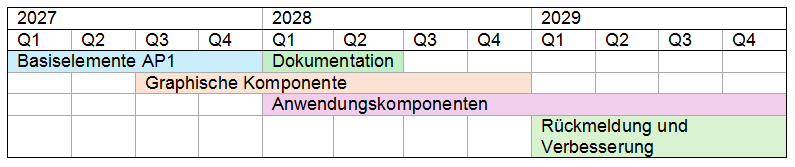
\includegraphics[width=\textwidth]{fig/osmbqc-gantt.png}
    \caption{Geplanter zeitlicher Ablauf des OSMBQC-Projektes.}
    \label{fig:gantt}
\end{figure}



\subsection{Risikomanagement}


Unter Annahme eines Projektbeginns zum 1.1.2027 kann ein Projektplan
wie folgt aufgestellt werden. Mit einem früheren oder späteren
Projektbeginn verschiebt sich der Zeitplan entsprechend.

\section{Wissenschaftliche und wirtschaftliche Anschlussfähigkeit, Ergebnisverwertung nach Projektende}

\instruction{Wichtigste Begründung für die Förderung! Wirtschaftliche
  und wissenschaftliche Nutzung.}

Die langfristige Verwendung des Simulationstools ermöglicht eine
Weiterentwicklung von messungsbasierten Quantenrechnen und seinen
verwandten Feldern.

Die Software wird sowohl im universitären Kontext als auch im Bereich
von Start-ups, KMUs und Großunternehmen mit Quantenbezug einen
Mehrwert erzeugen, da Ideen schneller umgesetzt werden können und
Schaltkreise und Lösungsansätze graphisch geteilt werden können.

Im Kontext des Open Innovation Ansatzes ist eine quelloffene
Weitergabe des Programms zur Weiterentwicklung von Komponenten ein
Ziel. Damit wird auch sichergestellt, dass die Software stets an den
gegenwärtigen Forschungsstand angepasst werden kann.


\section{Finanzierungsplan}

Der Finanzierungsplan ist in Anlage2\_Finanzen.xlsx zu finden.

Bei den Personalkosten kalkulieren wir mit zwei vollbeschäftigten
Wissenschaftlichen Mitarbeitern (TV-L E13, 100\%) sowie zwei
Wissenschaftlichen Hilfskräften (20h pro Woche) für Routineaufgaben.
Der Kostenansatz basiert auf den projektierten Personalkostensätzen
für die Jahre 2027-2029 die uns von der zentralen Verwaltung der LMU
München bereitgestellt wurden.

Für die Reisekosten planen wir mit zwei internationalen Reisen pro
Projektjahr.

\instruction{Bitte die Anlage ausfüllen und als separate Datei in
  elektronischer Form zusammen mit der Skizze einreichen. Bitte machen
  Sie dort unbedingt auf der vorgesehenen Seite entsprechende
  Anmerkungen zu den wichtigsten finanziellen Positionen. Ein grober
  Überblick reicht dabei, eine detaillierte Darstellung ist nicht
  notwendig.}

\bibliographystyle{alpha}
\bibliography{literatur}

\end{document}
